\documentclass{article}
\usepackage{listings}
\usepackage{color}
\usepackage{graphicx} 
\usepackage{float}
\usepackage{geometry}
\usepackage{subcaption}
\usepackage{todonotes}
\geometry{
    a4paper,
    total={170mm,257mm},
    left=15mm,
    right=15mm,
    top=15mm,
    bottom=15mm
}
\definecolor{codegreen}{rgb}{0,0.6,0}
\definecolor{codegray}{rgb}{0.5,0.5,0.5}
\definecolor{codepurple}{rgb}{0.58,0,0.82}

\definecolor{backcolour}{rgb}{0.95,0.95,0.92}
\lstdefinestyle{mystyle}{
    backgroundcolor=\color{backcolour},   
    commentstyle=\color{codegreen},
    keywordstyle=\color{magenta},
    numberstyle=\tiny\color{codegray},
    stringstyle=\color{codepurple},
    basicstyle=\ttfamily\footnotesize,
    breakatwhitespace=false,         
    breaklines=true,                 
    captionpos=b,                    
    keepspaces=true,                 
    numbers=left,                    
    numbersep=5pt,                  
    showspaces=false,                
    showstringspaces=false,
    showtabs=false,                  
    tabsize=2
}

\lstset{style=mystyle}

\title{Muestreo de Señal PWM}
\author{Oscar Ivan Moreno Gutierrez}
\date{\today}

\begin{document}

\maketitle

\section{Descripción}
Este proyecto se centra en realizar medidas sobre dos señales que se obtienen al filtrar una señal PWM generada con el dsPIC. Las medidas que se realizan incluyen el valor máximo, el valor medio y el valor eficaz de las señales. La información obtenida de ambas señales se muestra en una pantalla LCD. Además, se crea un filtro digital utilizando la herramienta de MATLAB para procesar las señales.
\section{Archivos y Directorios}
\begin{itemize}
\item \texttt{main.c}: Este es el archivo principal de mi proyecto.
\item \texttt{pintar\_lcd.c}: Este archivo se utiliza para funciones relacionadas con la visualización LCD.
\item \texttt{funciones.c}: Este archivo contiene funciones basicas y necesarias para el proyecto, como la aplicacion de filtros.
\end{itemize}



\section{Procedimiento}
Empezamos con la creacion de las funciones basicas del dsPIC utilizando un SSCP para una salida PWM, Cumpliendo el con el esquema proporcionado (Figura \ref{fig:esquema}).

\begin{figure}[H]
    \centering
    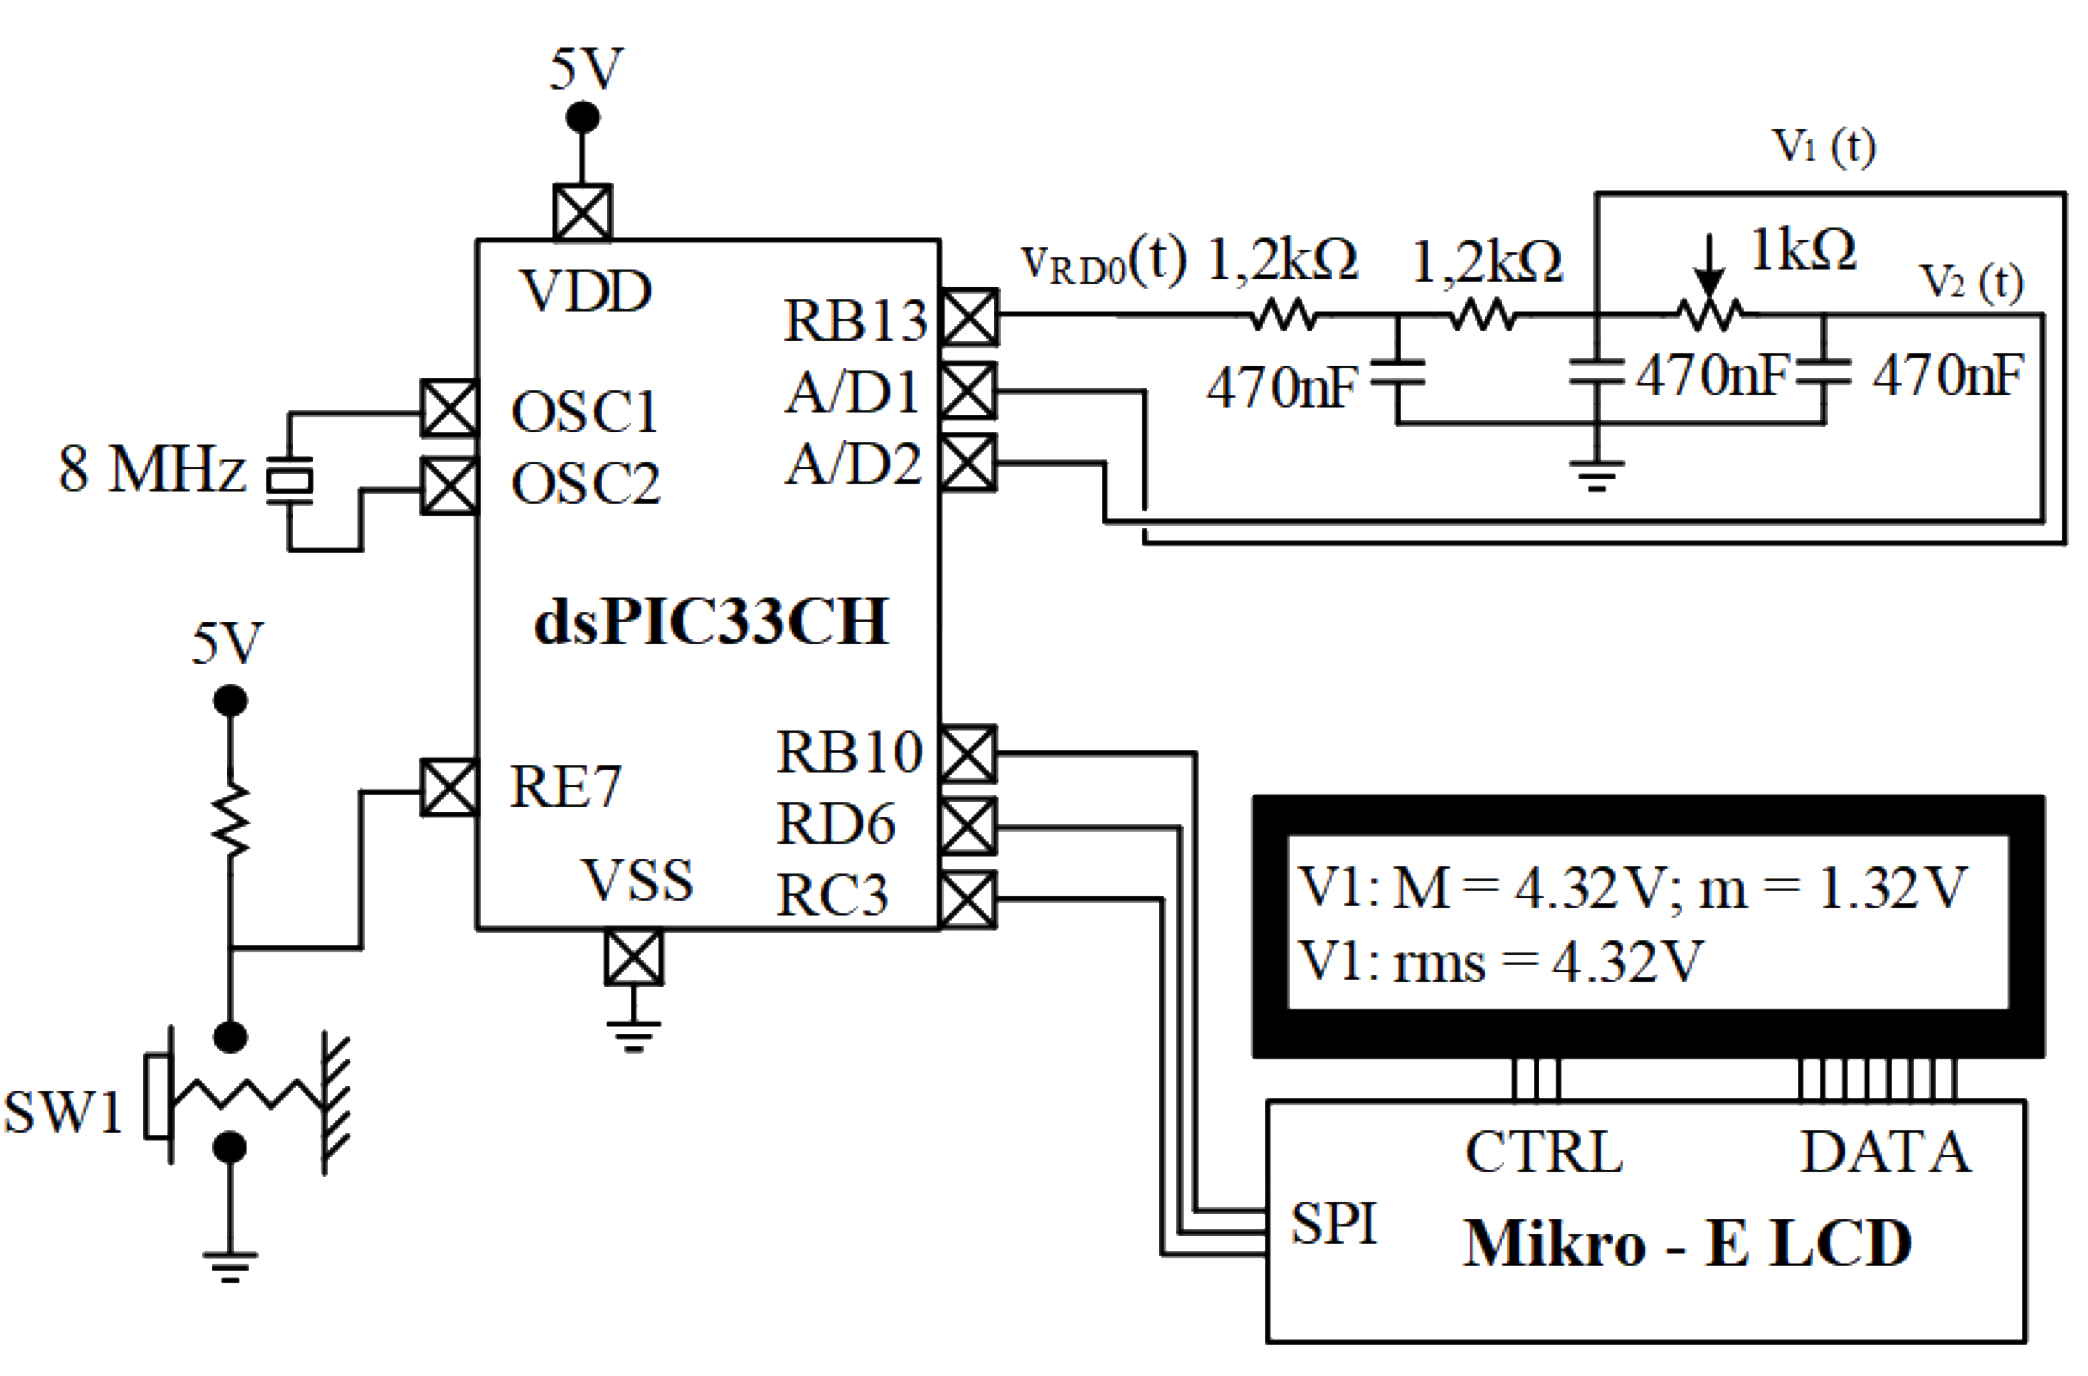
\includegraphics[width=0.5\textwidth]{images/esquema_og.png} % Replace with the path to your image
    \caption{Esquema del proyecto}
    \label{fig:esquema}
\end{figure}
La salida PWM sale por el RB13 y se conecta con un filtro proporcionado por el profesor.Donde se obtienen las señales senoidal y triangular.
Ademas de otros cambios:
\begin{itemize}
    \item El pin RE9 (Switch 3) sale de la pantalla de inicio.
    \item El pin RE8 (Switch 2) cambia el tipo de filtro aplicado.
    \item El pin RE7 (Switch 1) cambia el tipo de señal visualizada.
    \item El pin RA0 (potenciometro) se utiliza para manipular el ciclo de trabajo de la señal PWM.
    \item El pin RC1 fue asignado para ADC1, que recibe la señal senoidal.
    \item El pin RC3 fue asignado para ADC2, que recibe la señal triangular.
\end{itemize}
    Una mejora seria la implementacion de manipular el ciclo de trabajo con un modulo ADC. Utilizando un potenciometro para manipular el ciclo de trabajo de la señal PWM.

\subsection{Señales}
Posteriormente, realizo las medidas de las señales PWM,visualizado en un osciloscopio. Como se muestra en la Figura \ref{fig:osciloscopio}.
\begin{figure}[H]
    \centering
    \begin{subfigure}{.3\textwidth}
        \centering
        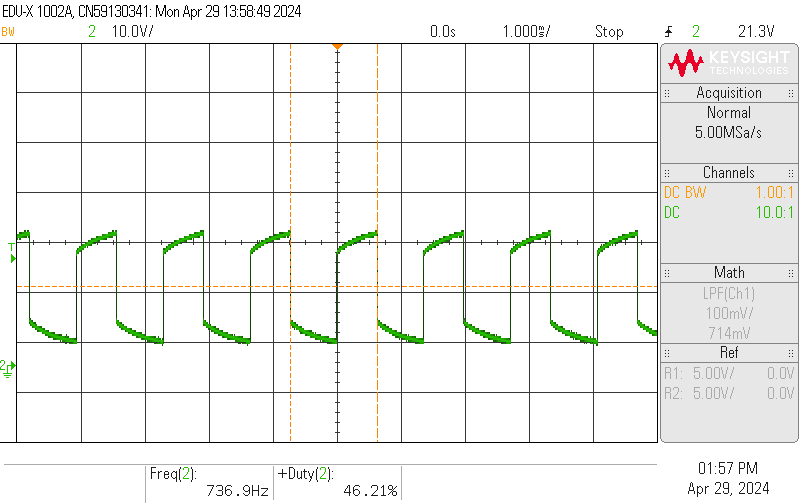
\includegraphics[width=\linewidth]{images/scope_1.png}
        \caption{Ciclo de trabajo 46\%}
        \label{fig:pwm_1}
    \end{subfigure}%
    \hfill
    \begin{subfigure}{.3\textwidth}
        \centering
        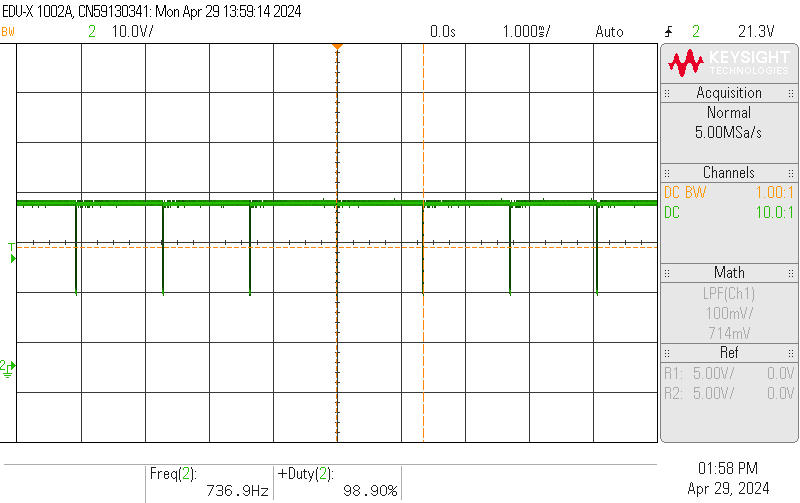
\includegraphics[width=\linewidth]{images/scope_2.png}
        \caption{Ciclo de trabajo 99\%}
        \label{fig:pwm_2}
    \end{subfigure}
    \hfill
    \begin{subfigure}{.3\textwidth}
        \centering
        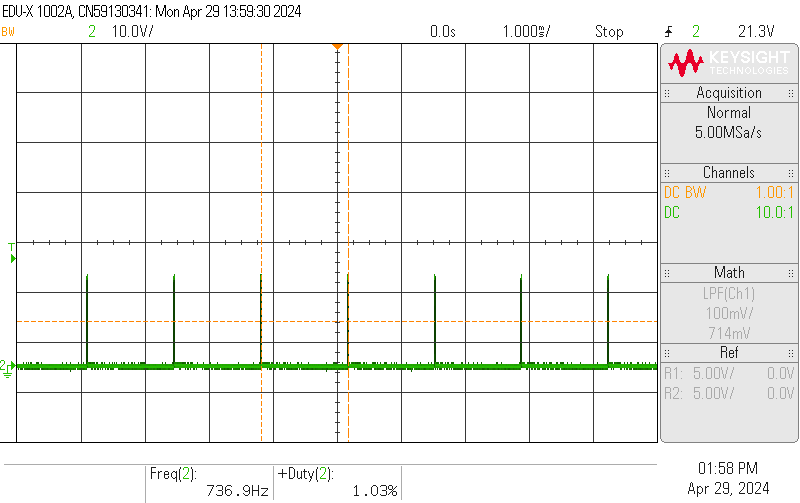
\includegraphics[width=\linewidth]{images/scope_3.png}
        \caption{Ciclo de trabajo 1\%}
        \label{fig:pwm_3}
    \end{subfigure}
    \caption{señal PWM en osciloscopio}
    \label{fig:osciloscopio}
\end{figure}
Se diseño que el limite de la señal PWM sea de 1\% a 99\% en su ciclo de trabajo. Se observa que la señal PWM se comporta de manera correcta en el osciloscopio.

La visualización de la señal senoidal se muestra en la Figura \ref{fig:senoidal}.

\begin{figure}[H]
    \centering
    \begin{subfigure}{.3\textwidth}
        \centering
        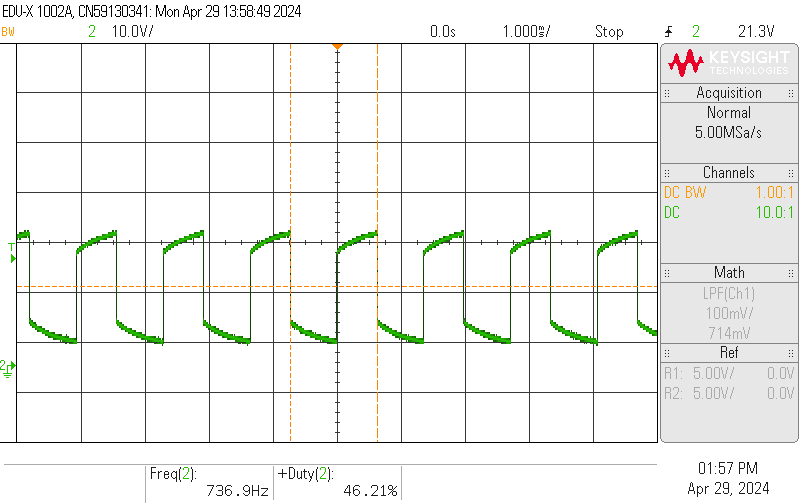
\includegraphics[width=\linewidth]{images/scope_1.png}
        \caption{Ciclo de trabajo 46\%}
        \label{fig:senoidal_1}
    \end{subfigure}%
    \hfill
    \begin{subfigure}{.3\textwidth}
        \centering
        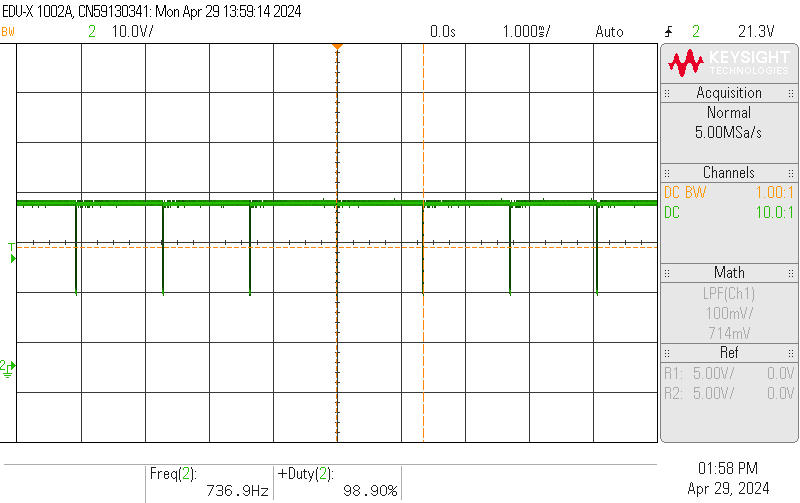
\includegraphics[width=\linewidth]{images/scope_2.png}
        \caption{Ciclo de trabajo 99\%}
        \label{fig:senoidal_2}
    \end{subfigure}
    \hfill
    \begin{subfigure}{.3\textwidth}
        \centering
        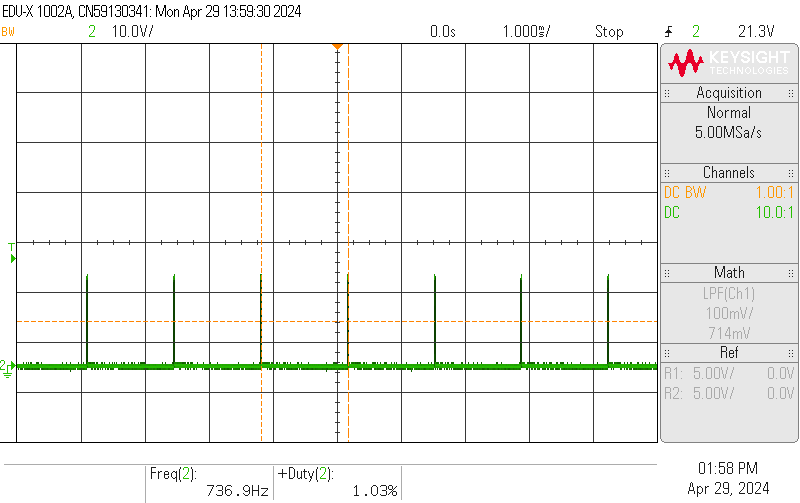
\includegraphics[width=\linewidth]{images/scope_3.png}
        \caption{Ciclo de trabajo 1\%}
        \label{fig:senoidal_3}
    \end{subfigure}
    \caption{señal senoidal en osciloscopio}
    \label{fig:senoidal}
\end{figure}
\todo{change the images correctly}
La visualización de la señal triangular se muestra en la Figura \ref{fig:triangular}.

\begin{figure}[H]
    \centering
    \begin{subfigure}{.3\textwidth}
        \centering
        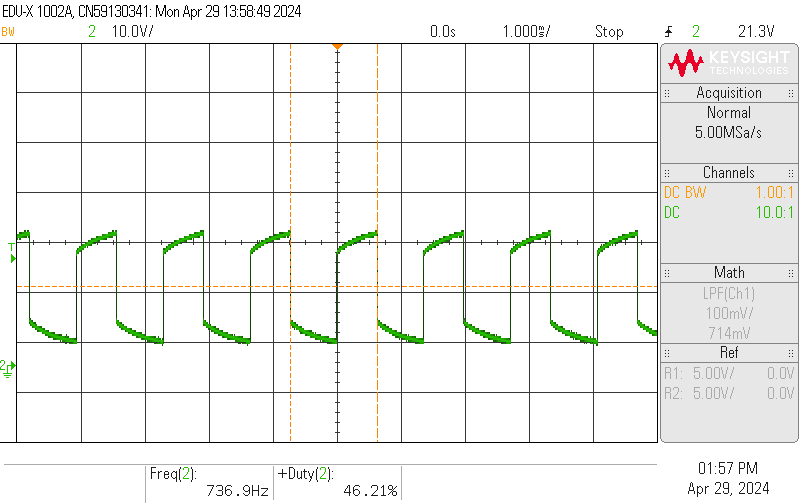
\includegraphics[width=\linewidth]{images/scope_1.png}
        \caption{Ciclo de trabajo 46\%}
        \label{fig:triangular_1}
    \end{subfigure}
    \hfill
    \begin{subfigure}{.3\textwidth}
        \centering
        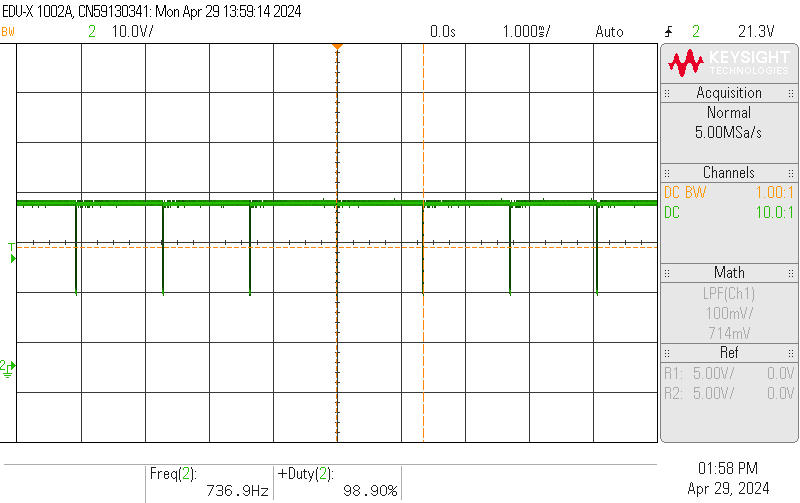
\includegraphics[width=\linewidth]{images/scope_2.png}
        \caption{Ciclo de trabajo 99\%}
        \label{fig:triangular_2}
    \end{subfigure}
    \hfill
    \begin{subfigure}{.3\textwidth}
        \centering
        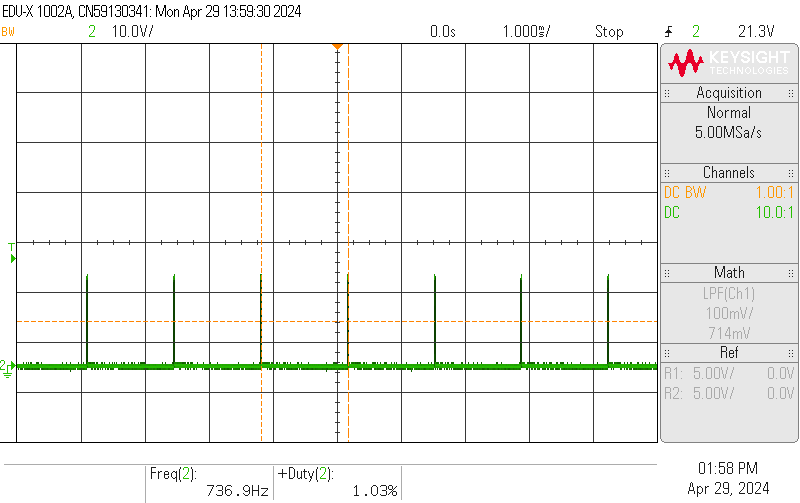
\includegraphics[width=\linewidth]{images/scope_3.png}
        \caption{Ciclo de trabajo 1\%}
        \label{fig:triangular_3}
    \end{subfigure}
    \caption{señal triangular en osciloscopio}
    \label{fig:triangular}
\end{figure}
\todo{change the images correctly}
\subsection{Filtros}
Se implemento un filtro digital a las señales senoidal y triangular. Se utilizo la herramienta de MATLAB Filter Desginer para diseñar el filtro. 
Primero conociendo la escogiendo una frecuencia adecuada de muestreo por la siguiente formula:
\begin{equation}
    f_s = 16 * 737 hz = 11792 Hz
\end{equation}
Donde 737 Hz es la frecuencia de nuestras señales.
Se obtuvo el siguiente filtro FIR:
\begin{itemize}
    \item \textbf{Filtro FIR}:Window
    \item \textbf{Frecuencia de muestreo}:  11792 Hz
    \item \textbf{Frecuencia de corte 1}: 710 Hz
    \item \textbf{Frecuencia de corte 2}: 750 Hz
    \item \textbf{Orden del filtro}: 50
    \item \textbf{Tipo de filtro}: Bandpass
\end{itemize}

Aplicacion para el Señal senoidal:
\begin{figure}[H]
    \centering
    \begin{subfigure}{.3\textwidth}
        \centering
        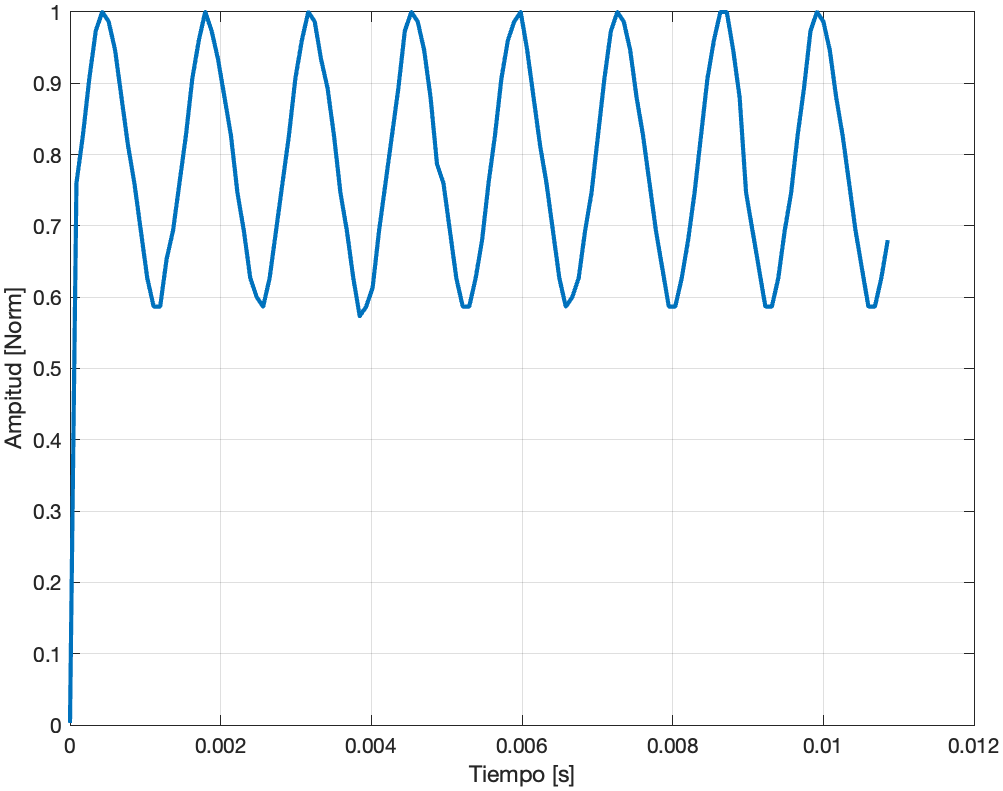
\includegraphics[width=\linewidth]{images/V1_entrada.png}
        \caption{Señal de entrada con respecto al tiempo}
        \label{fig:triangular_1}
    \end{subfigure}
    \hfill
    \begin{subfigure}{.3\textwidth}
        \centering
        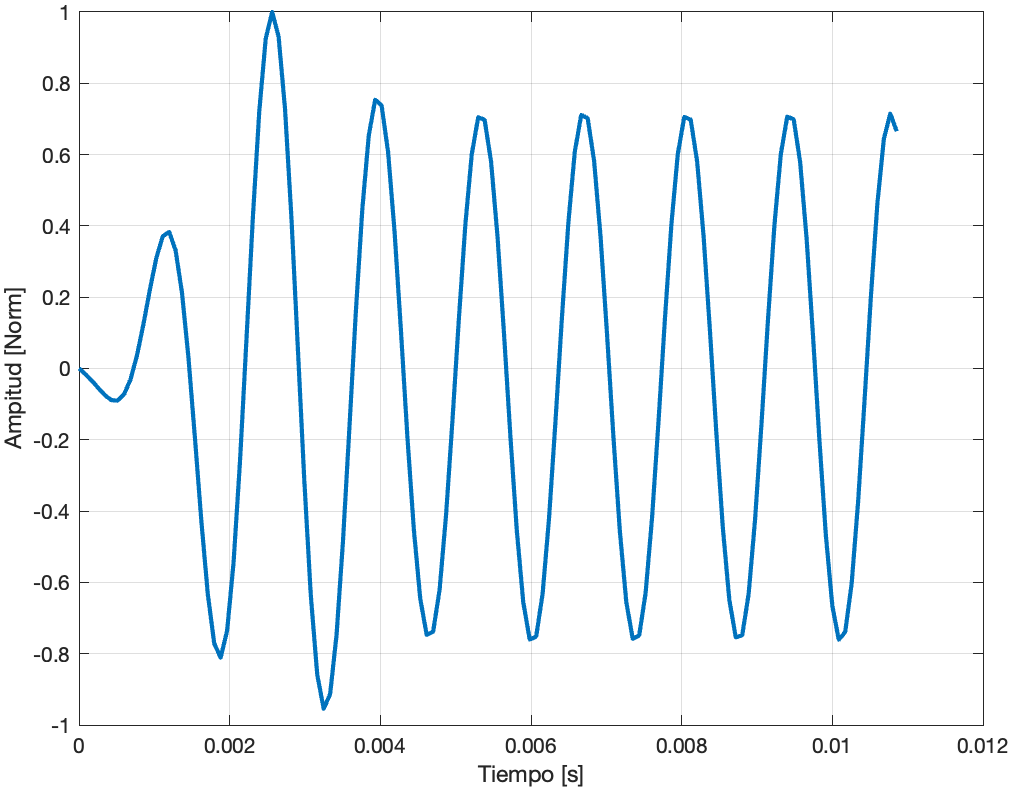
\includegraphics[width=\linewidth]{images/V1_Salida.png}
        \caption{Señal filtrada con respecto al tiempo}
        \label{fig:triangular_2}
    \end{subfigure}
    \hfill
    \begin{subfigure}{.3\textwidth}
        \centering
        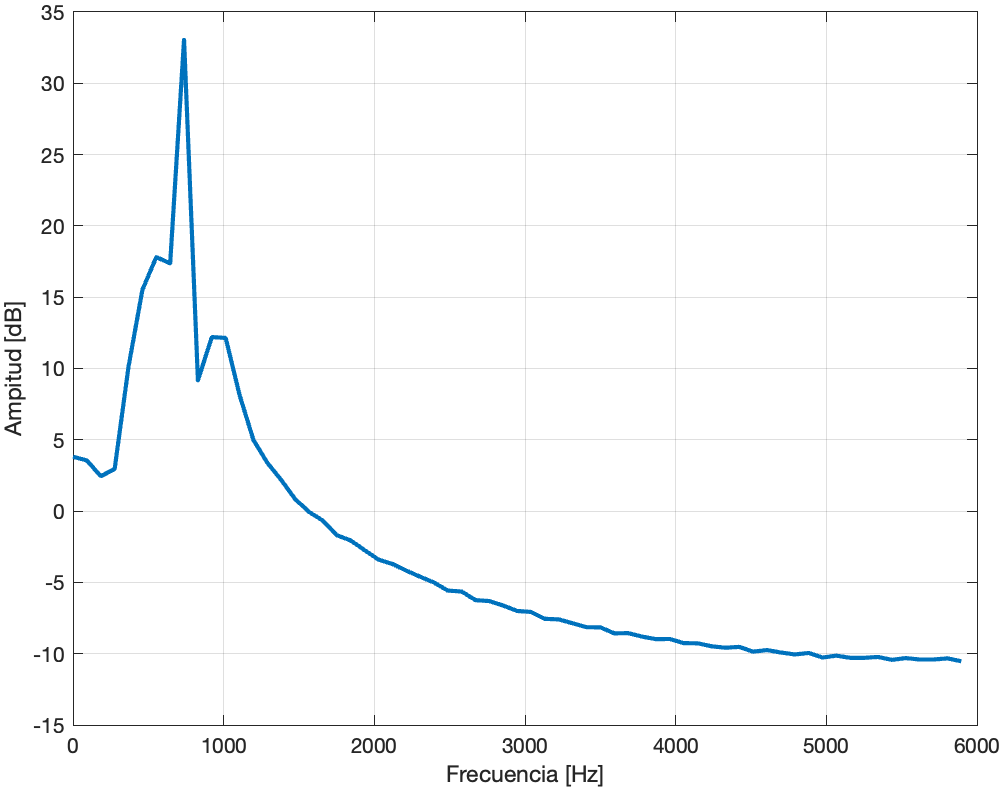
\includegraphics[width=\linewidth]{images/V1_Espectro.png}
        \caption{Espectro de la señal filtrada}
        \label{fig:triangular_3}
    \end{subfigure}    
    \caption{Filtro aplicado a la señal senoidal}
    \label{fig:senoidal_filtro}
\end{figure}

Aplication para la señal triangular:
\begin{figure}[H]
    \centering
    \begin{subfigure}{.3\textwidth}
        \centering
        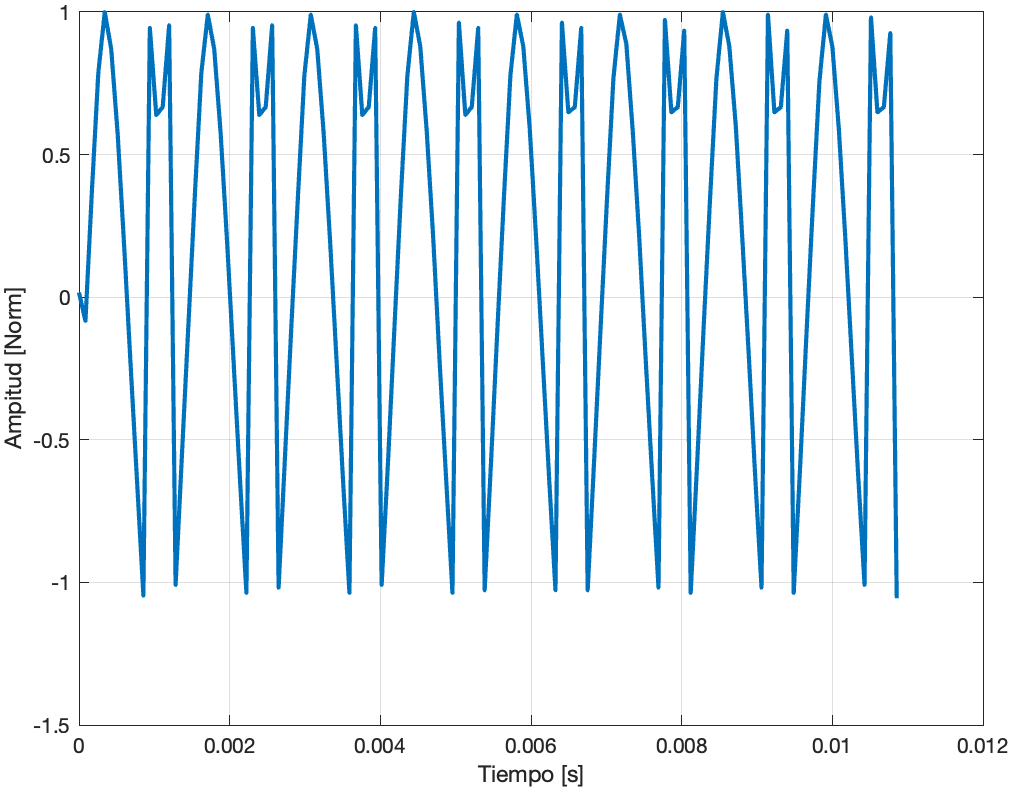
\includegraphics[width=\linewidth]{images/V2_entrada.png}
        \caption{Señal de entrada con respecto al tiempo}
        \label{fig:triangular_1}
    \end{subfigure}
    \hfill
    \begin{subfigure}{.3\textwidth}
        \centering
        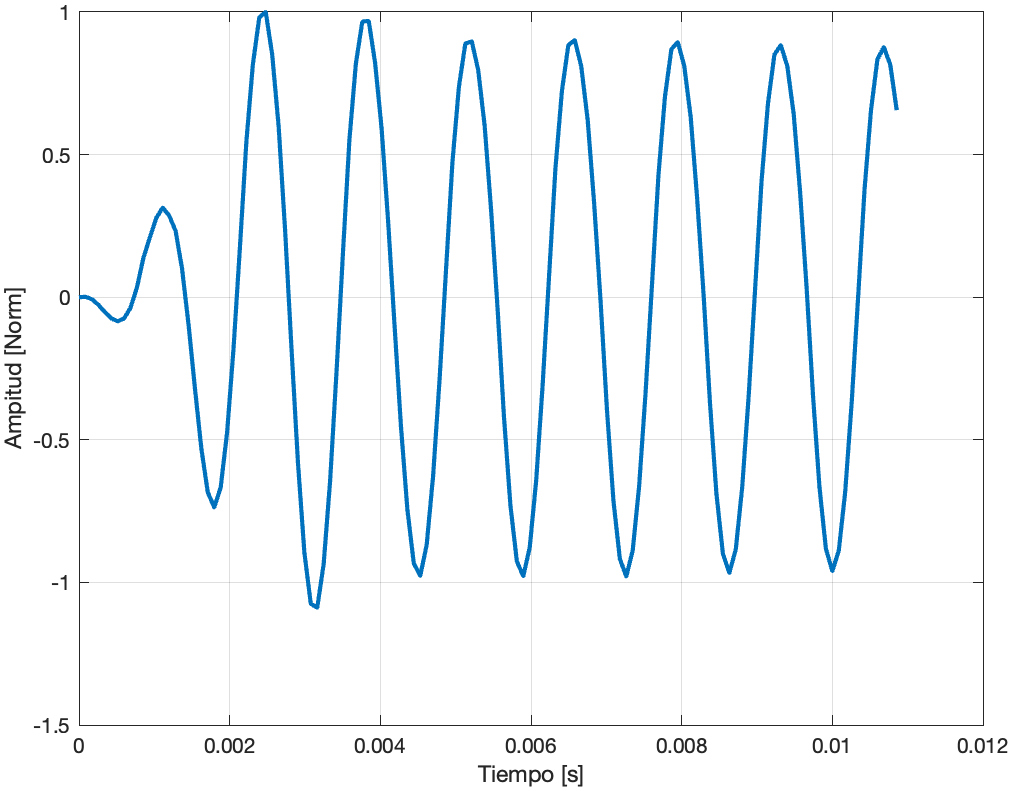
\includegraphics[width=\linewidth]{images/V2_Salida.png}
        \caption{Señal filtrada con respecto al tiempo}
        \label{fig:triangular_2}
    \end{subfigure}
    \hfill
    \begin{subfigure}{.3\textwidth}
        \centering
        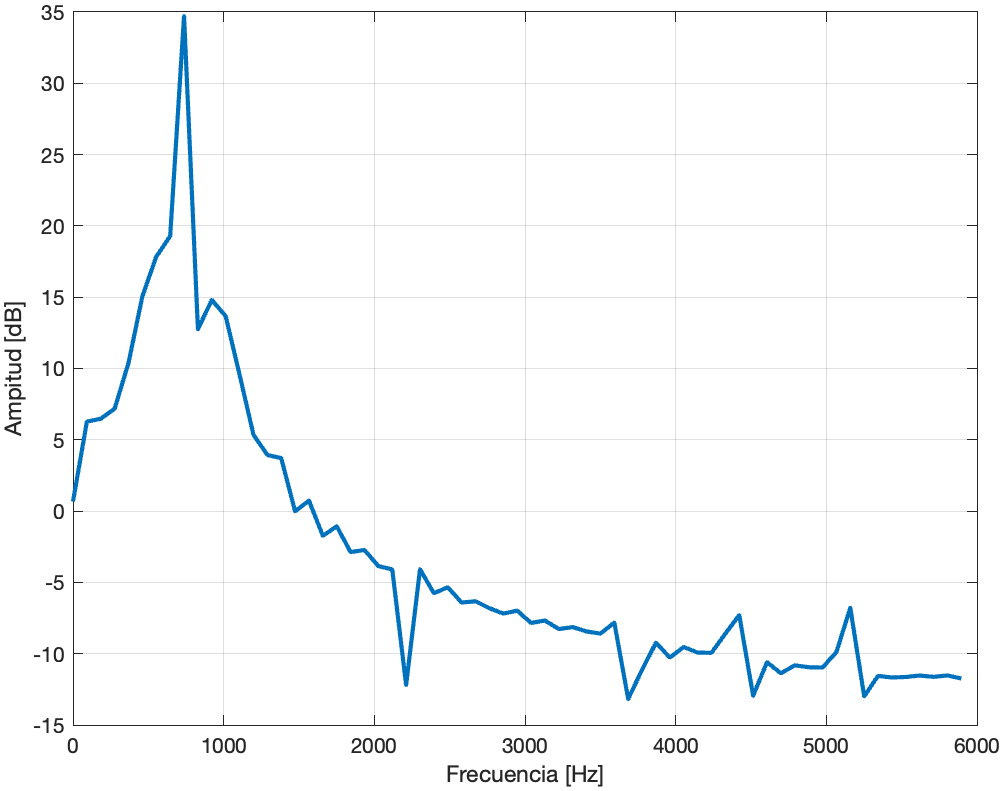
\includegraphics[width=\linewidth]{images/V2_Espectro.png}
        \caption{Espectro de la señal filtrada}
        \label{fig:triangular_3}
    \end{subfigure}    \caption{Filtro aplicado a la señal triangular}
    \label{fig:triangular_filtro}
\end{figure}

\section{Código}
\todo {explicar unas partes del codigo}
Para calcular el RMS:
\begin{lstlisting}[language=C]
    -----------------funciones.c-----------------
    float calculate_rms(int16_t* samples, uint8_t num_samples) {
    float sum_squared = 0.0;
    float mean_squared=0.0;
    float rms=0.0;
    for (uint8_t i = 0; i < num_samples; i++) 
        sum_squared += (float)samples[i] * (float)samples[i];
    mean_squared = sum_squared / num_samples;
    rms = sqrt(mean_squared);
    return rms;
}
\end{lstlisting}
Para aplicar el filtro FIR:
\begin{lstlisting}[language=C]
    --------------------main.c-------------------
    // multiplicacmos por 0x0100 para convertir a fractional
    buffer_fractional[buffer_move] = buffer[buffer_move] * 0x0100;
    aplicarFiltroFIR(buffer_fractional,buffer_filter,NUM_SAMPLES);
    // dividimos por 0x0100 para convertir a integer
    buffer[buffer_move] = buffer_filter[0] / 0x0100;
    -----------------funciones.c-----------------
    void aplicarFiltroFIR (fractional* buffer,fractional* output, uint8_t num_samples){
    extern FIRStruct FIR11792Filter;
    FIRDelayInit (&FIR11792Filter); 
    FIR(num_samples, &output[0], &buffer[0], &FIR11792Filter);
    return; 
 }
\end{lstlisting}

\end{document}